\chapter{2013 - PHYSICS 2A ACTUAL PRACTICAL A}

\begin{enumerate}
\item[1.] You are provided with a metre rule, a knife edge, two strings of length 100 cm each and two weights $W_1$ and $W_2$ of masses 50 g and 100 g respectively. Proceed as follows:
\begin{enumerate}
\item[(a)] Balance a metre rule on a knife edge, put a mark and write G at the balancing point using a piece of chalk or a pencil. Measure and record the length $l$, width $w$ and thickness $t$ of a metre rule using a vernier caliper.
\item[(b)] Place the metre rule on a knife edge so that the knife edge is at 60 cm of your metre rule (see Figure 1 (a)). Suspend weight $W_2$ of 100 g on the right hand side of the knife edge. Adjust $W_2$ until the metre rule balances horizontally. Read and record lengths `b' and `c' as seen in Figure 1 (a).

\begin{center}
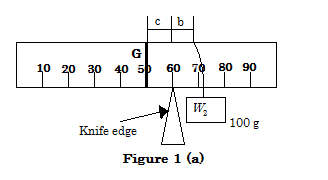
\includegraphics[width=9cm]{./img/2013-1a-alt.png}
\end{center}

\begin{enumerate}
\item[(i)] Suspend weight $W_1$ of 50 g on the left hand side of the knife edge at the position 47 cm and adjust weight $W_2$ until the metre rule balances horizontally as seen in Figure 1 (b). Read and record the lengths `a' and `b'.

\begin{center}
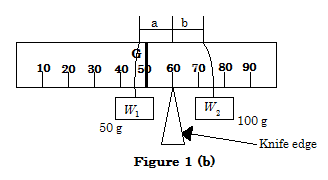
\includegraphics[width=9cm]{./img/2013-1b-alt.png}
\end{center}

\item[(ii)] Repeat the procedures in (b) (i) by adjusting the position of $W_1$ to the left at the interval of 3 cm to obtain other four (4) readings.
\end{enumerate}
\item[(c)] Tabulate your results as shown in Table 1.\\

\quad Table 1\\
\quad \quad \begin{tabular}{|p{4cm}|p{4cm}|} \hline
\multicolumn{1}{|c|}{a (cm)} & \multicolumn{1}{c|}{b (cm)} \\ \hline
& \\ \hline
& \\ \hline
\end{tabular}\\[10pt]

\item[(d)] Plot a graph of ``b'' against ``a''.
\item[(e)] What is the nature of the graph?
\item[(f)] Calculate the slope $S$ of the graph.
\item[(g)]
\begin{enumerate}
\item[(i)] Read the $b$-intercept, given that $b = Sa + \cfrac{W}{W_2} \times c$
\item[(ii)] What does $\left(\cfrac{W}{W_2}\right)c$ represent in your graph?
\item[(iii)] Calculate the value of $W$ using the relation $W_2 = \cfrac{Wc}{9.5 \text{cm}}$. What does $W$ represent?
\end{enumerate}
\item[(h)]
\begin{enumerate}
\item[(i)] Find the value of the ratio $P = \cfrac{l \times w \times t}{m}$.
\item[] \textbf{Note:} The mass $m$ of a meter rule can be obtained by calculations.
\item[(ii)] What is the physical meaning of the value of $P$?
\end{enumerate}
\item[(i)] State a possible source of error in this experiment.
\item[(j)] How can you minimize error in 1 (i)?
\item[(k)] State the aim of this experiment.
\end{enumerate}
\end{enumerate}
\flushright \textbf{(25 marks)}
\flushleft

\begin{enumerate}
\item[2.] You are provided with a Plane mirror, a Ruler, Protract, Drawing board, Optical pins, Office pins and Plain papers. Proceed as follows:
\begin{enumerate}
\item[(a)] On the plain paper provided, draw a line 13 cm from the top of the paper and call it M$_1$M$_2$. Pin your paper on the board provided and place the reflecting surface of the mirror along the line M$_1$M$_2$ as seen in Figure 2.

\begin{center}
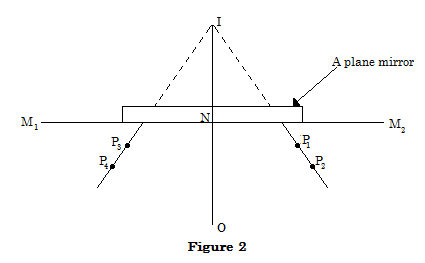
\includegraphics[width=10cm]{./img/2013-2-alt.png}
\end{center}

\item[(b)] Insert pin O as an object at 4.0 cm in front of the mirror. Place pins P$_1$ and P$_2$ so as to appear in one straight line with the image of object O seen in the plane mirror.
\item[(c)] Remove pins P$_1$ and P$_2$, using other pins, place pins P$_3$ and P$_4$ so as to appear in a straight line with the image of object O in the other side (see Figure 2).
\item[(d)] Remove the mirror and pins. Draw lines joining P$_1$ and P$_2$ on one side and the other joining P$_3$ and P$_4$ on the other side of object O, extend both lines to meet at I on the other side of line M$_1$M$_2$.
\item[(e)] Join OI, a line cutting the reflecting surface at N.
\item[(f)] Repeat this procedure for the distance of an object being 6, 8, 10 and 12 cm.
\item[(g)] On all the diagrams drawn:
\begin{enumerate}
\item[(i)] Measure the distance ON and NI.
\item[(ii)] Comment on the distances obtained in 2 (g) (i).
\item[(iii)] What is the nature of image? Give reasons for your answer.
\item[(iv)] State four characteristics of the image you obtained.
\item[(v)] What is the aim of this experiment?
\item[(vi)] Mention and state the law governing this experiment.
\item[(vii)] Explain a source of error in this experiment.
\item[(viii)] How can you minimize the error in (vii) above?\\

\item[] \textbf{Note:} The papers used for drawing should be attached and collected together with answer booklets.
\end{enumerate}
\end{enumerate}
\end{enumerate}
\flushright \textbf{(25 marks)}
\flushleft